\scanpage{29}
\uline{Lemme} Soit $\deleted{\unsure{\mathcal X|X}}K$ un arrangt 1-dimensionnel de \inserted{$N$} ps. droites, sans ps. droites bigonales, avec $N\geq5$. Alors on peut ordonner ces $D_1\ldots D_N$, de telle façon que, si $K_i$ désigne l'\unsure{arrangt|arrangement} défini par $D_1\ldots D_i$, alors, pour

$1^\circ)$ $D_1$ -- $D_4$ de type $\mathrm{II}_4$ \deleted{\unsure{ou}} (\deleted{resp.} $D_1$ -- $D_6$ type $\mathrm{III}_6$)

$2^\circ)$ Pour $i\geq5$ \inserted{(resp. $i\geq7$)}, $D_i$ non bigonal dans $K_i$. \deleted{(resp. pour $i\geq7$, $D_i$ \unsure{non}} (NB Dans le cas \unsure{respé|resp.|inverse}, \deleted{\unsure{c'est}} $2^\circ)$ est automatique. \unsure{\}} \deleted{\unsure{NPS que|UPS que}} Dans le \deleted{$K_5$} cas non respé, on peut supposer que $K_5$ est du type $\mathrm{II}_5$, ou du type $\mathrm{II}_{3,2}$, et que les autres types \inserted{$K_i$ $(i\geq6)$} sont $\mathrm{II}_{pq}$, et dans le cas $\mathrm{III}_6$ on peut supposer que $K$ lui-même est $\mathrm{III}_6$, ou $\mathrm{IV}_7$. Pour lemme plus précis,

% slanted
\margin{cas mutuellement exclusifs}
\[\left\{\begin{aligned}
&\text{Ou bien }\exists\, K_5\text{ du type }\mathrm{II}_5\\
&\text{Ou bien }\exists\, K_5\text{ du type }\mathrm{II}_{32},\\
&\text{Ou bien }\deleted{\exists}K\simeq\mathrm{III}_6\text{ ou }\mathrm{IV}_7,
\end{aligned}\right.\]
\margin{-- et quand on continue à rajouter des ps droites $1:1$, c'est pas des bigones}
\margin{et $K$ de type $\mathrm{II}_{pq}$ et alors, quand on rajoute ps-droite, jamais bigonale}
\margin{donc $\exists\,K_6\simeq\mathrm{III}_6$, et \deleted{\unsure{D'}} dans le cas $\mathrm{III}_7$, si on rajoute une ps. droite, elle n'est pas bigonale}

Les pts de départ sont \unsure{de} \deleted{\unsure{telle}} \unsure{façons} $\mathrm{II}_4$ ou $\mathrm{III}_6$.
\figure{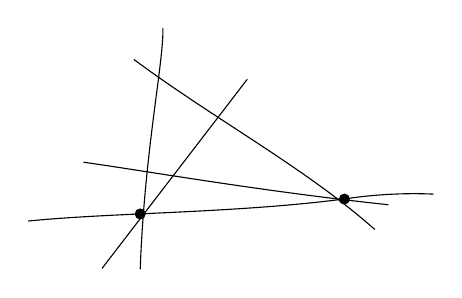
\begin{tikzpicture}[x=.009cm,y=-.009cm]
\draw (2,277) .. controls (120,265) and (293,266) .. (447,246) .. controls (486,240) and (530,237) .. (574,239);
\draw (192,5) .. controls (193,54) and (166,179) .. (160,345);
\draw (106,344) -- (311,77);
\draw (151,49) .. controls (264,133) and (393,202) .. (491,289);
\draw (80,194) .. controls (172,207) and (331,235) .. (510,254);
\fill (160,267) circle[radius=2pt];\fill (448,246) circle[radius=2pt];
\end{tikzpicture}}
% archive sheet number: 28
